\documentclass[tikz,border=3pt]{standalone}
\usepackage[T1]{fontenc}
\usepackage{times}
\usepackage{xcolor}
\usepackage{tikz}
\usetikzlibrary{arrows.meta,positioning}

\definecolor{huntrixblue}{HTML}{1F5A7A}
\definecolor{huntrixteal}{HTML}{2A8C82}
\definecolor{huntrixgold}{HTML}{D59B32}
\definecolor{huntrixred}{HTML}{B5483A}
\definecolor{huntrixgray}{HTML}{EEF2F4}

\begin{document}
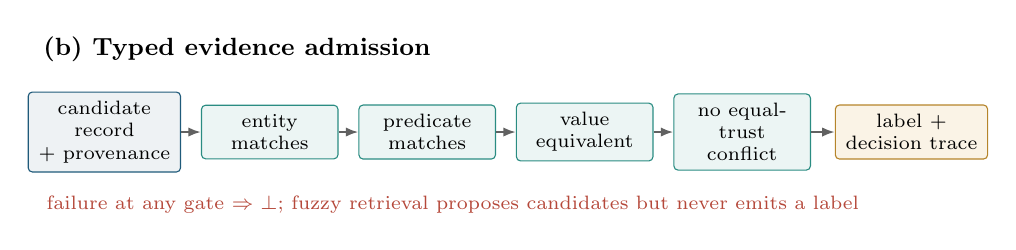
\begin{tikzpicture}[
  every node/.style={font=\scriptsize},
  box/.style={draw=huntrixblue, rounded corners=1.5pt, fill=huntrixgray,
              minimum height=6.8mm, align=center, text width=17mm},
  gate/.style={draw=huntrixteal, rounded corners=1.5pt, fill=huntrixteal!9,
               minimum height=6.8mm, align=center, text width=15mm},
  outcome/.style={draw=huntrixgold!85!black, rounded corners=1.5pt,
                  fill=huntrixgold!12, minimum height=6.8mm,
                  align=center, text width=17mm},
  arrow/.style={-{Latex[length=1.6mm]}, thick, draw=black!62}
]
\node[font=\small\bfseries, anchor=west] at (0,1.05) {(b) Typed evidence admission};
\node[box] (record) at (0.9,0) {candidate record\\+ provenance};
\node[gate] (entity) at (3.0,0) {entity\\matches};
\node[gate] (predicate) at (5.0,0) {predicate\\matches};
\node[gate] (value) at (7.0,0) {value\\equivalent};
\node[gate] (conflict) at (9.0,0) {no equal-trust\\conflict};
\node[outcome] (emit) at (11.15,0) {label +\\decision trace};
\draw[arrow] (record) -- (entity);
\draw[arrow] (entity) -- (predicate);
\draw[arrow] (predicate) -- (value);
\draw[arrow] (value) -- (conflict);
\draw[arrow] (conflict) -- (emit);
\node[anchor=west, text width=104mm, align=center, text=huntrixred] at (0,-0.92)
  {failure at any gate $\Rightarrow\bot$; fuzzy retrieval proposes candidates but never emits a label};
\end{tikzpicture}
\end{document}
